\documentclass{beamer}
\usepackage{graphicx}
\usepackage{graphics}
\usepackage{hyperref}
\usepackage[english]{babel}
\usepackage[T1]{fontenc}
\usepackage[utf8]{inputenc}
\usepackage{xfrac}
\usepackage{array}
\usepackage{multirow}
\usepackage[normalem]{ulem}


\mode<presentation>
{
    \usetheme{AMUFree-kk}
    \setbeamercovered{transparent = 28}
}
\title{We need go \sout{deeper} bigger}
\date{2022}
\author{Karol Kaczmarek}
\setbeamertemplate{bibliography item}{[\theenumiv]}


\begin{document}

\begin{frame}
    \titlepage
\end{frame}

\iffalse
\AtBeginSection[]
{
    \begin{frame}
        \frametitle{Outline}
        \tableofcontents[currentsection]
    \end{frame}
}
\fi

\begin{frame}
    \begin{center}
        
\includegraphics[scale=3.25]{img/meme_we_need_go_deeper_bigger.png}
    \end{center}
\end{frame}

\begin{frame}
    \begin{center}
        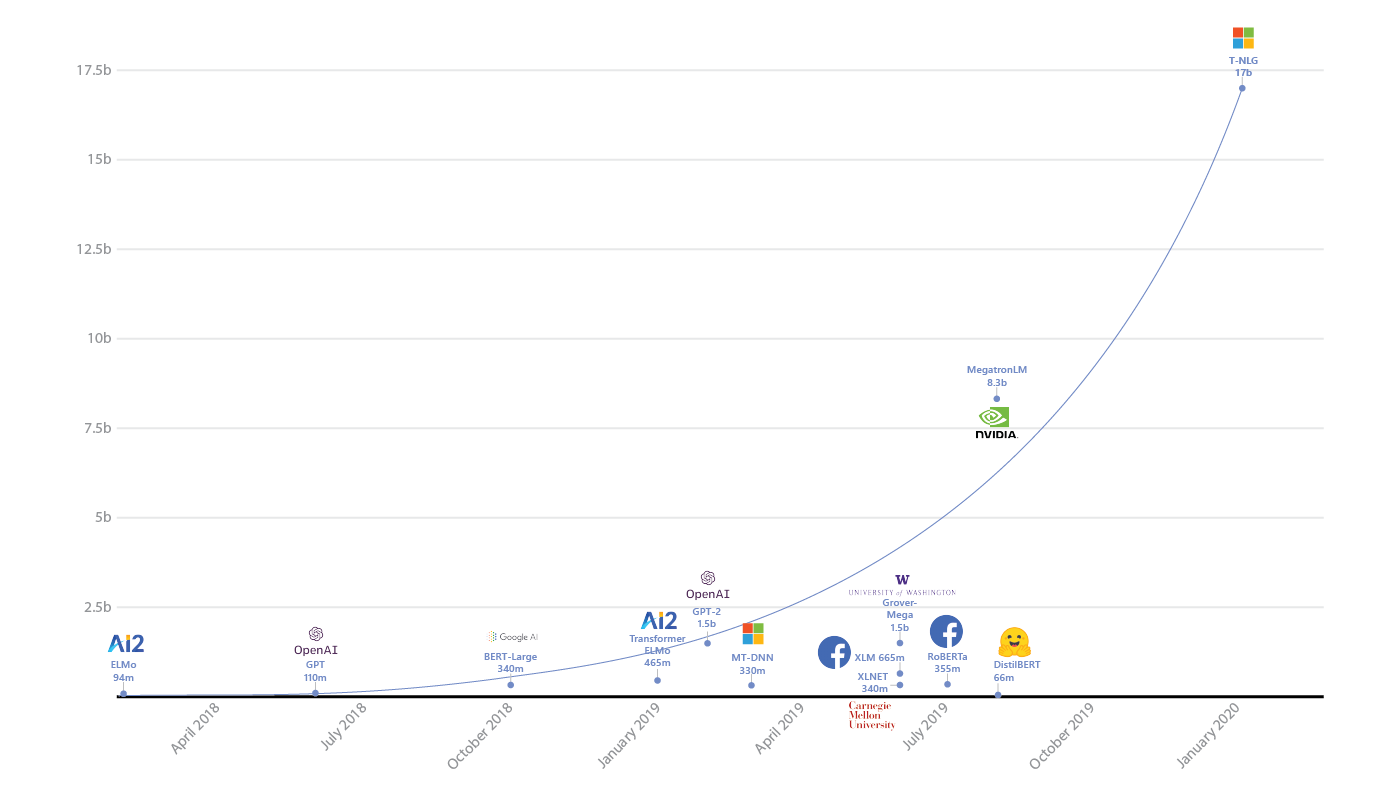
\includegraphics[scale=0.245]{img/TurningNGL.png}
    \end{center}
    \tiny{TuringNGL - Januray 2020}
\end{frame}

\begin{frame}
    \begin{center}
        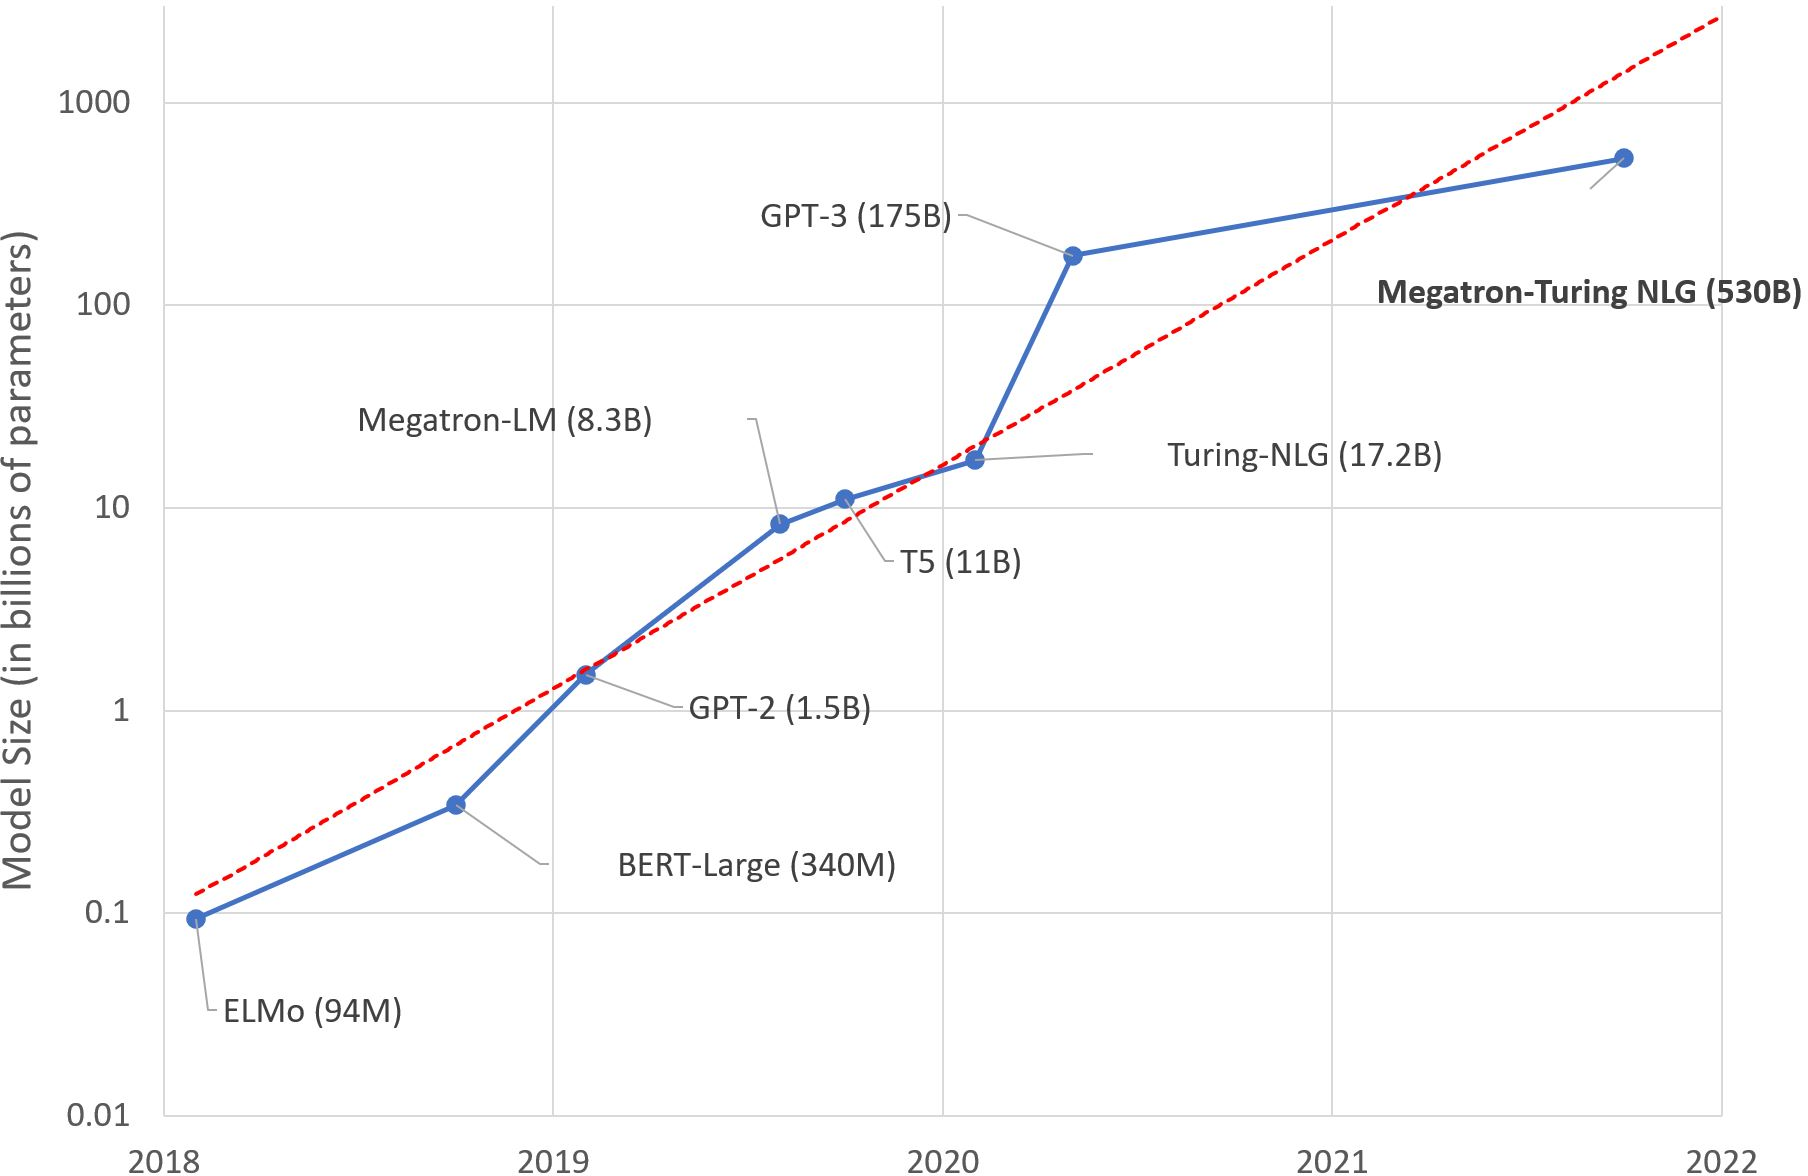
\includegraphics[scale=0.725]{img/MT-NLG.png}
    \end{center}
    \tiny{MT-NLG - October 2021}
\end{frame}

\begin{frame}
    \frametitle{Data Parallelism (DP)}
    \begin{itemize}
        \item model parameters are replicated on each device
        \item at each step, a mini-batch is divided evenly across all the data parallel processes
        \item each process executes the forward and backward propagation on a different subset of data samples
        \item use of averaged gradients across processes to update the model locally
        \item torch.nn.DataParallel, torch.nn.parallel.DistributedDataParallel
    \end{itemize}
\end{frame}

\begin{frame}
    \frametitle{Model Parallelism (MP)}
    \begin{itemize}
        \item splits the model vertically, partitioning the computation and parameters in each layer across multiple devices
        \begin{itemize}
        \item \textbf{Tensor Model Parallelism} - partitions the individual layers of the model across workers
        \item \textbf{Pipeline Model Parallelism} - divides the layers of the model into stages that can be processed in parallel
        \end{itemize}
        \item requiring significant communication between each layer
        \item manual splitting, Gpipe \cite{gpipe}, Pipedream \cite{pipedream}, Mesh-Tensorflow \cite{mesh_tensorflow}, Megatron-LM \cite{megatronlm} \cite{megatronlm_2}, L2L \cite{l2l}, Zero \cite{zero} \cite{zero_offload} \cite{zero_infinity}, JAX \cite{jax} + Haiku \cite{jax_haiku} (library for JAX), torch.distributed.fsdp.FullyShardedDataParallel \cite{blog_torch_fsdp}
    \end{itemize}
\end{frame}

\begin{frame}
    \frametitle{Data Parallelism (DP) and Model Parallelism (MP)}
    \begin{center}
        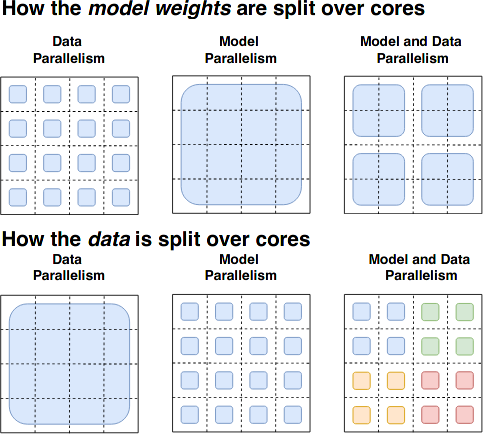
\includegraphics[scale=0.42]{img/data_distribution.png}
    \end{center}
\end{frame}

% Gopher
\begin{frame}
    \frametitle{Gopher \cite{gopher}}
    \begin{itemize}
        \item December 2021, Google/DeepMind - JAX and Haiku
        \item analysis of Transformer-based language model performance across a wide range of model scales and \textbf{152 diverse tasks}
        \item train 6 models: 44M, 117M, 417M, 1.4B, 7.1B, 280B (called \textbf{Gopher})
        \item achieving state-of-the-art (SOTA) of 100/124 tasks (only 124 tasks has published LM performance)
        \item analysis of the training dataset and model behavior, covering the intersection of model scale with bias and toxicity, wide range of analyzes (120 page vs. 75 pages GPT-3)
    \end{itemize}
\end{frame}

\begin{frame}
    \frametitle{Architecture}
    \begin{itemize}
        \item 280B \textbf{autoregressive} Transformer (decoder) with modifications:
        \begin{itemize}
            \item use \textbf{RMSNorm} (root mean square layer normalization) instead of LayerNorm
            \item use the \textbf{relative positional encoding} (allows evaluate on longer sequences than was trained)
        \end{itemize}
        \item 2048 tokens in sequence length
        \item \textbf{32k} byte-level SentencePiece vocabulary
        \item train for 300 billion tokens
        \item mixed precision (bfloat16) training with stochastic rounding
        \item using Adam optimizer (instead of Adafactor - instabilities of pre-training larger models)
    \end{itemize}
\end{frame}

\begin{frame}
    \frametitle{Models}
    \begin{center}
        \begin{tabular}{ l | c | c | c | c | c }
        \textbf{Model} & \textbf{Layers} & \textbf{Heads} & \textbf{$d_{model}$} & \textbf{Max LR} & \textbf{Batch} \\
        & & & & & \textbf{Size} \\
        \hline
        44M  & 8  & 16  & 512   & $6 \times 10^{-4}$ & $0.25$M \\
        117M & 12 & 12  & 768   & $6 \times 10^{-4}$ & $0.25$M \\
        417M & 12 & 12  & 1536  & $2 \times 10^{-4}$ & $0.25$M \\
        1.4B & 24 & 16  & 2048  & $2 \times 10^{-4}$ & $0.25$M \\
        7.1B & 32 & 32  & 4096  & $1.2 \times 10^{-4}$ & $2$M \\
        \hline
        280B & 80 & 128 & 16384 & $4 \times 10^{-5}$ & $3$M $\rightarrow$ $6$M$^{1}$ \\
        Gopher & & & & & \\
        \hline
        175B & 96 & 96  & 12288 & $0.6 \times 10^{-4}$ & $3.2$M \\
        GPT-3 & & & & & \\
        \end{tabular}
    \end{center}

    \tiny{$^{1}$ - after warm up}
\end{frame}

\begin{frame}
    \frametitle{Training}
    \begin{itemize}
        \item use \textbf{JAX pmap} transformation to efficiently express both data and model parallelism
        \item trained and evaluated all models on TPUv3 chips
        \item \textbf{half-precision} parameters and \textbf{single-precision} Adam state for Gopher occupy \textbf{2.5 TiB} (16 GiB of memory in TPUv3 core)
        \item use \textbf{optimiser state partitioning, model parallelism} and \textbf{rematerialisation} (checkpointing) to partition the model state and reduce the activations
        \item create \textbf{MassiveText} (web pages, books, news articles and code)
    \end{itemize}
\end{frame}

\begin{frame}
    \frametitle{Lower-Precision Training}
    \begin{center}
        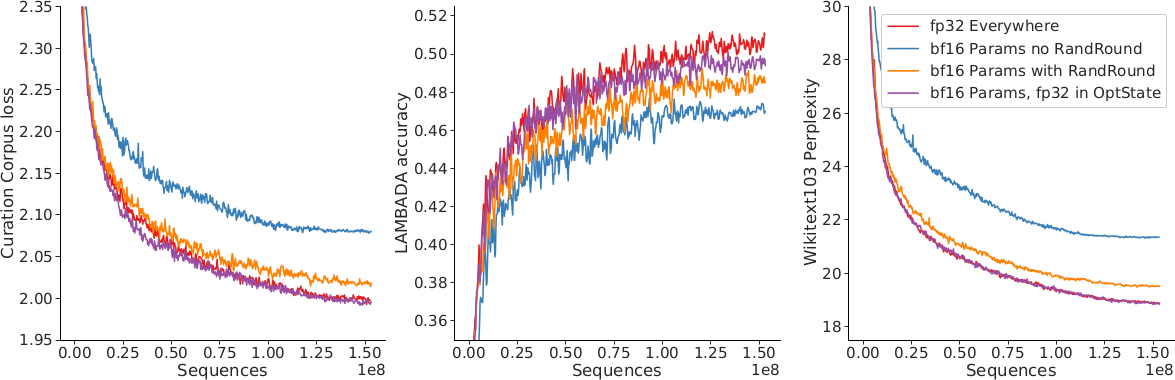
\includegraphics[scale=1.1]{img/fp16.png}
    \end{center}
    \begin{itemize}
        \tiny{\item \textbf{fp32}: Significand precision: 24 bits, Exponent width: 8 bits}
        \tiny{\item \textbf{fp16}: Significand precision: 11 bits, Exponent width: 5 bits}
        \tiny{\item \textbf{bf16}: Significand precision: 8 bits, Exponent width: 8 bits}
    \end{itemize}
\end{frame}

\begin{frame}
    \frametitle{Lower-Precision Training}
    \begin{itemize}
        \item \textbf{fp32 Everywhere} - both parameters and activations are stored in fp32
        \item \textbf{bf16 parameters without Random Rounding} - parameters and activations are cast to bp16, no random rounding during the parameter update
        \item \textbf{bf16 parameters with Random Rounding} - parameters and activations are cast to bf16, random rounding during the parameter update
        \item \textbf{bf16 parameters with a fp32 copy in the partitioned optimiser state} - parameters and activations are cast to bf16, copy of the parameters are stored in
fp32 in the optimiser state and used for the update, parameters are randomly rounded to bf16 for the forward pass
    \end{itemize}
\end{frame}

\begin{frame}
    \frametitle{Train data}
    \begin{center}
        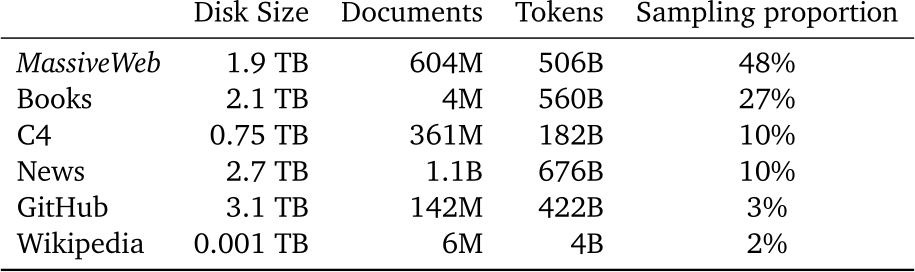
\includegraphics[scale=1.5]{img/gopher_train_data.png}
    \end{center}
\end{frame}

\begin{frame}
    \frametitle{Evaluation data}
    \begin{center}
        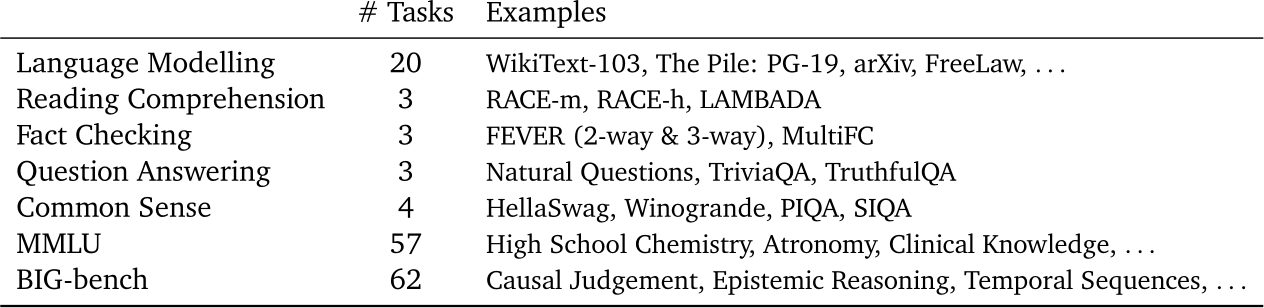
\includegraphics[scale=1.12]{img/gopher_eval_data.png}
    \end{center}
\end{frame}

\begin{frame}
    \frametitle{And much much more}
    About \textbf{60 pages} of additional analysis...
\end{frame}


% GShard
\section{GShard}
\begin{frame}
    \frametitle{GShard \cite{gshard} -- MoE (Mixture-of-Experts)}
    \begin{itemize}
        \item June/July 2020, Google
        \item parallel computation patterns with \textbf{minimal changes} to the existing model code
GShard enabled us to scale up multilingual neural machine translation Transformer model with Sparsely-Gated Mixture-of-Experts beyond \textbf{600B parameters} using automatic sharding
        \item train 600B model on 2048 TPU v3 accelerators in 4 days to achieve far superior quality for translation from 100 languages to English
        \item even train 1 trillion model (\textbf{problem with stability training}, did not include the results)
    \end{itemize}
\end{frame}

\begin{frame}
    \frametitle{Sparsely-Gated Mixture-of-Experts Transformer (MoE Transformer)}
    \begin{center}
        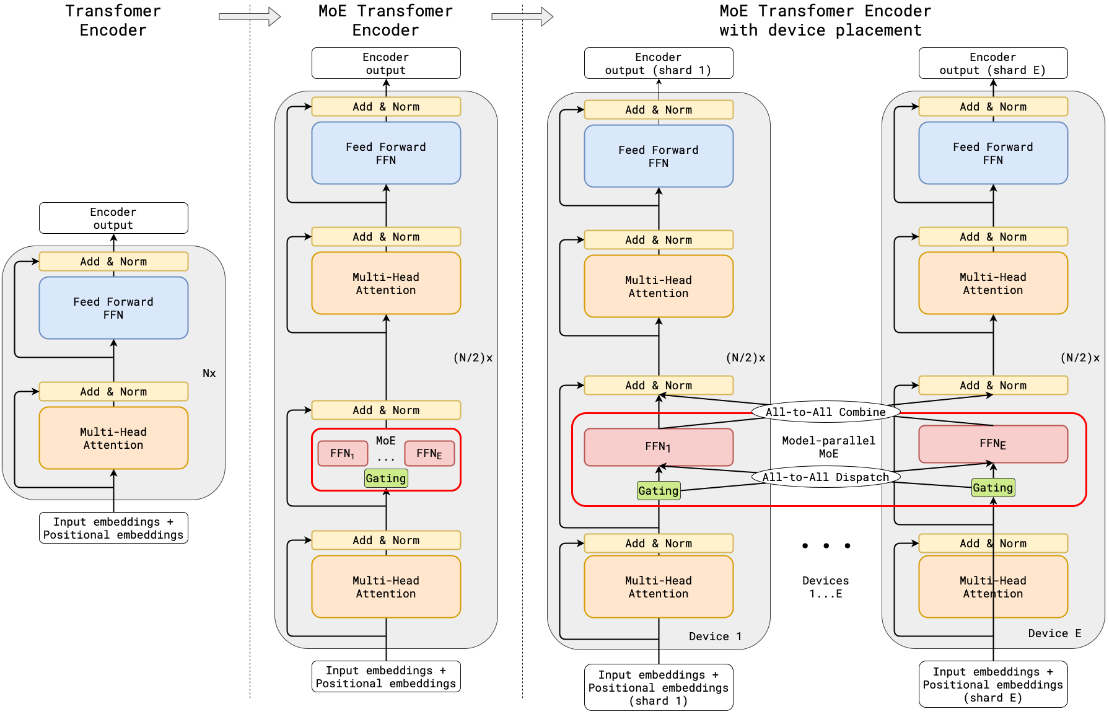
\includegraphics[scale=0.25]{img/gshard_architecture.png}
    \end{center}
\end{frame}




% ZeRO
\section{ZeRO}
\begin{frame}
    \frametitle{ZeRO \cite{zero} -- DeepSpeed}
    \begin{itemize}
        \item October 2019 (blogs - February 2020 \cite{blog_turing_nlg}), Microsoft - PyTorch
        \item Turing-NLG - Turing Natural Language Generation - 17 billion parameters
        \item ZeRO (Zero Redundancy Optimizer) - optimize \textbf{memory}, vastly improving \textbf{training speed} while increasing \textbf{the model size} that can be efficiently trained, constains two sets of optimizations:
        \begin{itemize}
            \item \textbf{ZeRO-DP} (ZeRO-powered data parallelism) aimed at reducing the memory footprint of the model states (removes the memory state redundancies across data-parallel processes by \textbf{partitioning} the model states instead of \textbf{replicating})
            \item \textbf{ZeRO-R} targeted towards reducing the residual memory consumption (\textbf{activation} partitioning
with CPU offloading, appropriate size for \textbf{temporary buffers}, preventing \textbf{memory fragmentation})
        \end{itemize}
    \end{itemize}
\end{frame}

% ZeRO-Offload
\section{ZeRO-Offload}
\begin{frame}
    \frametitle{ZeRO-Offload \cite{zero_offload} -- DeepSpeed}
    \begin{itemize}
        \item January 2021, Microsoft - PyTorch
        \item train models with over 13 billion parameters on a single GPU (Nvidia V100 32GB)
        \item offload the \textbf{gradients, optimizer states and optimizer} computation to CPU, while keeping the parameters and
forward and backward computation on GPU
        \item reduce CPU compute time while maximizing memory savings on GPU to their existing training pipeline (\textbf{Fast CPU Adam optimizer} and \textbf{One-Step Delayed Parameter Update})
    \end{itemize}
\end{frame}

% ZeRO-Infinity
\section{ZeRO-Infinity}
\begin{frame}
    \frametitle{ZeRO-Infinity \cite{zero_infinity} -- DeepSpeed}
    \begin{itemize}
        \item April 2021, Microsoft - PyTorch
        \item \textbf{ZeRO-Infinity} - heterogeneous system technology that leverages GPU, CPU, and NVMe memory to allow for unprecedented model scale on limited resources without requiring model code refactoring
        \item available through DeepSpeed (ZeRO-Infinity extends the ZeRO with new innovations in heterogeneous memory access called the \textbf{infinity offload engine})
        \item running 32 trillion parameters on 32 NVIDIA DGX-2 nodes (512 V100 GPUs)
        \item supports 1 trillion parameters per NVIDIA V100 DGX-2 node - 50x increase over 3D parallelism
    \end{itemize}
\end{frame}

% Megatron-LM
\section{Megatron-LM}
\begin{frame}
    \frametitle{Megatron-LM \cite{megatronlm_2}}
    Megatron-LM (April 2021 - Nvidia) - train 1 trillion parameters  on 3072 GPUs (Nvidia A100 80GB - 384 DGX A100 nodes):
    \begin{center}
        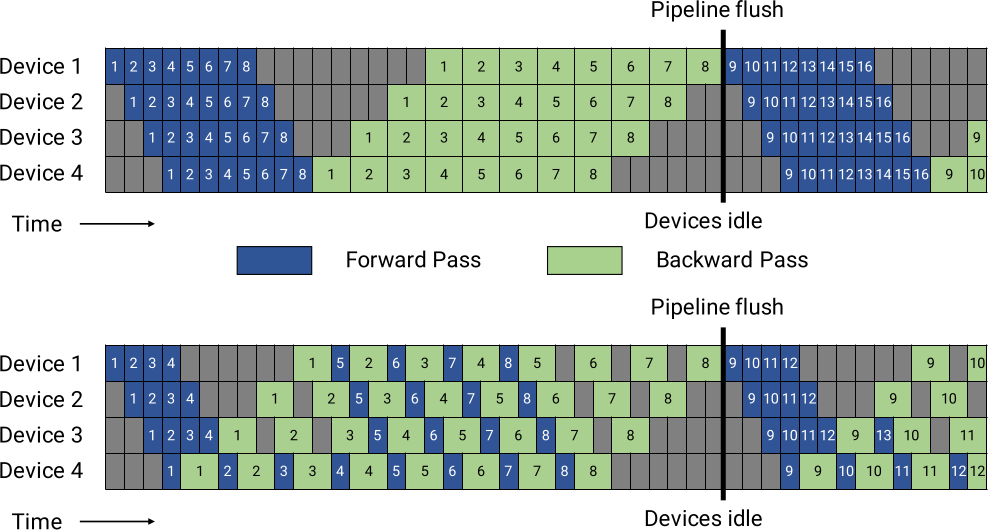
\includegraphics[scale=1.05]{img/megatron_lm.png}
    \end{center}
    \tiny{and other optimizations (\textbf{activation checkpointing}, \textbf{CPU-offloading}, \textbf{adaptive optimization}).}
\end{frame}

% Megatron-Turing NLG
\begin{frame}
    \frametitle{Megatron-Turing NLG \cite{deepspeed_megatron}}
    \begin{itemize}
        \item January 2022 (blogs - October 2021 \cite{blog_mt_nlg}), Microsoft - PyTorch
        \item combines \textbf{pipeline parallelism and data parallelism from DeepSpeed} with \textbf{tensor-slicing from Megatron} to create \textbf{3D-parallelism}
        \item train \textbf{530B} model (Megatron-Turing NLG -- MT-NLG)
        \item use \textbf{280} Nvidia A100 GPUs (Nvidia Selene = 560 Nvidia A100):
        \begin{itemize}
        \item 8-way tensor-slicing within a node
        \item 35-way pipeline parallelism across nodes
        \end{itemize}
        \item achieves SOTA zero-shot, one-shot, and few-shot learning on several NLP benchmarks
    \end{itemize}
\end{frame}

\begin{frame}
    \frametitle{Architecture}
    \begin{itemize}
        \item 530B \textbf{autoregressive} Transformer (decoder): \textbf{105} Transformer layers, \textbf{20480} model dimensions and \textbf{128} attention heads
        \item \textbf{2048} tokens in sequence length and \textbf{1920} batch size
        \item train for 339 billion tokens
        \item mixed precision (bfloat16) training
        \item using Adam optimizer
        \item better weight initialization, lower learning rate (higher learning rate increases the model instability), better Adam parameters
    \end{itemize}
\end{frame}

\begin{frame}
    \frametitle{Models}
    \begin{center}
        \begin{tabular}{ l | c | c | c | c | c }
        \textbf{Model} & \textbf{Layers} & \textbf{Heads} & \textbf{$d_{model}$} & \textbf{Max LR} & \textbf{Batch} \\
        & & & & & \textbf{Size} \\
        \hline
        280B & 80 & 128 & 16384 & $4 \times 10^{-5}$ & $3$M $\rightarrow$ $6$M$^{1}$ \\
        Gopher & & & & & \\
        \hline
        175B & 96 & 96  & 12288 & $0.6 \times 10^{-4}$ & $3.2$M \\
        GPT-3 & & & & & \\
        \hline
        530B & 105 & 128  & 20480 & $5 \times 10^{-5}$ & - \\
        MT-NLG & & & & & \\
        \end{tabular}
    \end{center}

    \tiny{$^{1}$ - after warm up}
\end{frame}

\begin{frame}
    \frametitle{Train data}
    \begin{center}
        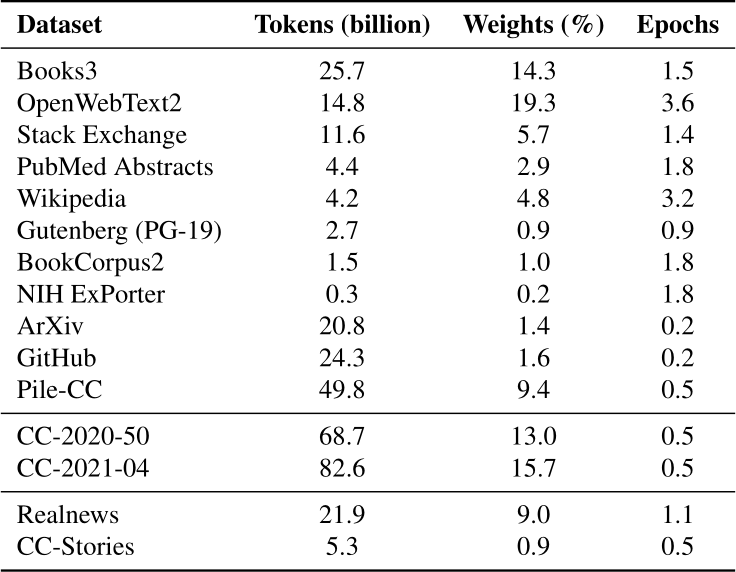
\includegraphics[scale=1.4]{img/mt_nlg_train_data.png}
    \end{center}
\end{frame}



% GPT-NeoX-20B
\section{GPT-NeoX-20B}
\begin{frame}
    \frametitle{GPT-NeoX-20B \cite{gpt_neox} \cite{blog_gpt_neox_20b}}
    \begin{itemize}
        \item Feburary 2022, EleutherAI - PyTorch
        \item the \textbf{largest publicly accessible} pretrained general-purpose autoregressive language model
        \item base on Megatron and DeepSpeed
        \item trained on the Pile (825GiB of raw text data)
        \item weights alone take up around \textbf{40GB} in GPU memory and, due to the tensor parallelism scheme as well as the high memory usage, you will need at \textbf{minimum 2 GPUs} with a total of \textbf{45GB} of GPU VRAM to run inference, and significantly more for training
    \end{itemize}
\end{frame}


\begin{frame}
    \frametitle{Architecture}
    The same as GPT-3 with changes:

    \begin{center}
        \begin{tabular}{ l | c | c }
        \textbf{Component} & \textbf{GPT-3} & \textbf{GPT-NeoX-20B} \\
        \hline
        Positional & Absolute & Rotary \\
        Embeddings & & \\
        \hline
        Parallel Attention & No & Yes \\
        + FF Layers & & \\
        \hline
        Sparse Layers & Yes & No \\
        \end{tabular}
    \end{center}

    $^{1}$ Rotary Positional Embeddings \cite{roformer} - twist embedding space so that the attention of a token at position $m$ to token at position $n$ is linearly dependent on $m-n$
\end{frame}



% Fine tune GPT-3 - follow instruction
% https://cdn.openai.com/papers/Training_language_models_to_follow_instructions_with_human_feedback.pdf

% XGLM
% Few-shot Learning with Multilingual Language Models
% https://github.com/pytorch/fairseq/tree/main/examples/xglm#pre-trained-models
% https://arxiv.org/abs/2112.10668
\section{Other}
\begin{frame}
    \frametitle{Other}
    \begin{itemize}
        \item \textbf{FLAN} \cite{flan} - 137B Transformer (like GPT-3), instruction tuning
        \item \textbf{XGLM} \cite{xglm} - 7.5B multilingual autoregressive Transformer, few-shot learning
        \item \textbf{PanGu} \cite{pangu} - 200B Chinese Transformer
        \item \textbf{LaMDA} \cite{lamda} - 137B Transformer specialized for dialog
        \item \textbf{DeepNet} \cite{deepnet} - scale Transformers up to 1000 layers
        \item \textbf{PolyCoder} \cite{polycoder} - 2.7B Transformer based on the GPT-2 architecture, multi-lingual corpus of code, Codex alternative -- GitHub Copilot
    \end{itemize}
\end{frame}


%PyTorch brazki z telefonu



% References
\section{References}
\begin{frame}[allowframebreaks,t]
    \tiny
    \frametitle{References}
    \bibliographystyle{ieeetr}
    \bibliography{large_models}
    %\nocite{*}
\end{frame}

\end{document}
